% !TEX root =  master.tex
\chapter{Grundlagen}
\section{Projektumfang}
Als Ausgangslage dient in diesem Projekt eine handelsübliches elektrisch öffenbares Garagentor, das mit einer Fernbedienung gesteuert wird. Dabei wird davon ausgegangen, dass es sich um eine 1-Kanal Steuerung handelt, also dass ein einmaliges Drücken eines Knopfes der Fernbedienung das Garagentor öffnet und ein weiteres Betätigen desselben Knopfes das Garagentor wieder schließt. Weiterhin wird davon ausgegangen, dass das Garagentor beim Auftreffen auf ein Hindernis automatisch reversiert. Dies ist sogar, wie durch ein Gerichtsurteil des OLG Frankfurt von 2015 festgestellt, gesetzlich vorgeschrieben. %#TODO https://openjur.de/u/775737.html
Die Ansteuerung und Regelung des Garagentor-Motors selbst sind also nicht Bestandteil dieser Projektarbeit.

Neben der automatisierten Öffnung durch die Kennzeichenerkennung wurden folgende Features als Projektumfang festgelegt:

\begin{itemize}
\item Amazon Alexa oder Google Home Integration, um das Garagentor auch als "Fußgänger" und ferngesteuert öffnen zu können (um Gartengeräte zu entnehmen oder den Postboten ein Paket abstellen zu lassen)




\item Logging der Ein- und Ausfahrenden Fahrzeuge, um das Produkt eventuell später auch für kommerzielle Parkhäuser und Tiefgaragen nutzen zu können
\end{itemize}
Folgende Features wurden als optional festgehalten und deren Implementierung vom Projektverlauf abhängig gemacht:
\begin{itemize}
\item Lichtschranke zur Erkennung ob die Garage bereits belegt ist. In diesem Fall soll das Tor nicht geöffnet werden und es einem anderen Fahrzeug, das ebenfalls einfahrtsberechtigt ist, ermöglicht werden VOR der Garage zu parkieren ohne ständig durch das sichtbare Kennzeichen die automatische Öffnung auszulösen.

\item Öffnung per Transponder, um das Tor vor Ort und ohne Smartphone öffnen zu können, falls der Akku leer ist oder man anderen Personengruppen (evtl. temporären) Zutritt erteilen möchte
\end{itemize}

\section{Hardware}
Aufgrund der vielseitigen Verwendbarkeit, des geringen Preises, der guten Konnektivität und Kompatibilität wurde sich für ein Rasberry Pi 3+ bzw. 4 entschieden. Diese Modelle sind hervorragend für IoT-Anwendungen geeignet und verfügen mit 1 bzw. 4 oder 8 GB trotzdem über genug Arbeitsspeicher um einfache Bildverarbeitung durchführen zu können. 

Als einfachste Schnittstelle zum Torantrieb wurde der Handsender identifiziert. Hier genügt es zwei Drähte am Ein- und Ausgang des Aktivierungsknopfes anzulöten und diese mit einem Relais zu verbinden. Dann kann durch die \ac{GPIO}-Pins das Relais verbunden und geöffnet oder geschlossen werden und somit ein Betätigen der Fernbedienung simuliert werden.


\subsection{Raspberry Pi 3}
Der Raspberry Pi ist ein vollständiger Computer in der Größe einer Kreditkarte. Er wird von der nicht profitorientierten Raspberry Pi Foundation entwickelt und in Großbritannien hergestellt. Er besitzt keinen aufgelöteten Speicher, sondern bootet direkt von einer MicroSD-Karte. Die Raspberry Pi Foundation entwickelt auch das offizielle Betriebssystem Pi OS auf Basis von Linux (Debian).

Die Zweite Version des Raspberry Pi (3 Mod. B v1.2) hat 1GB RAM und als CPU vier ARM Cortex-A53-Kerne, welche die ARMv8-A-Mikroarchitektur implementieren. Für dieses Modell gibt es aktuell keine offizielle 64-bit-Version von Pi OS, was die Kompatibilität mit bestimmter Software einschränkt.
Die Schnittstellen umfassen MicroUSB für die Stromversorgung, HDMI für die Bildausgabe, 3,5mm Klinke für Audio, RJ-45 (Ethernet), 4x USB 2.0, 26 \ac{GPIO}-Pins und zwei Flachband-Header für den offiziellen Touchscreen und die offizielle Kamera.

Die vierte Version (4 Mod. B) hat eine schnellere CPU mit vier ARM Cortex-A72-Kernen, 4GB RAM, fest verbautes Wi-fi und bluetooth sowie zwei Micro-HDMI-Buchsen. Die Form ist gleich geblieben.

\subsection{Luxonis OAK-D}
Die Luxonis OAK-D ist eine IoT-Kamera, die einen RGB-Sensor und ein Paar Stereosensoren hat. Der Stereosensor nutzt einen Sony IMX378-Sensor und kann Video in 4k aufnehmen. Das Stereopaar nutzt Omnivision OV9282-Sensoren mit einer Auflösung von 1280x800.
Die Sensoren sind direkt mit der integrierten Myriad X-VPU verbunden. Stromversorgung und Datentransfer erfolgen über USB-C, wobei sowohl USB 2.0 als auch USB 3.0 unterstützt werden.

Die Kamera wird über die DepthAI-Platform und deren Python-API gesteuert. Hierbei kann der Entwickler selbst entscheiden, welche Sensoren und Funktionen der VPU er in welchem Ausmaß nutzt.\autocite[Vgl.][]{oakd}

Als Vision Processing Unit verwendet die OAK-D den Myriad X der Intel-Tochterfirma Movidius ist eine \ac{VPU}, die auf IoT-Anwendungen spezialisiert ist. Sie unterstützt bis zu 8 Kameras mit einer Auflösung von 4k. Sie kann Aufgaben wie Stereosicht und Bildverarbeitung sehr effizient ausführen und ist dabei nicht auf Datentransfers zu externem Speicher angewiesen.

Zusätzlich ist sie mit einer Neural Compute Engine ausgestattet, die ein schnelles und Energieeffizientes Ausführen von Inferenz auf neuralen Netzen ermöglicht. Movidius gibt eine Performance von 1 TOPS (1 Billion Operationen pro Sekunde) an.

Der eingebaute Myriad X ist eine \ac{VPU}, die auf IoT-Anwendungen spezialisiert ist. Sie unterstützt bis zu 8 Kameras mit einer Auflösung von 4k. Sie kann Aufgaben wie Stereosicht und Bildverarbeitung sehr effizient ausführen und ist dabei nicht auf Datentransfers zu externem Speicher angewiesen.

Zusätzlich ist sie mit einer Neural Compute Engine ausgestattet, die ein schnelles und Energieeffizientes Ausführen von Inferenz auf neuralen Netzen ermöglicht. Movidius gibt eine Performance von 1 TOPS (1 Billion Operationen pro Sekunde) an.
\subsection{RC522 RFID-Modul}

Das RC552-Modul von NXP Semiconductors ist ein RFID-Transponder, der das 13.56Mhz ISM-Band nutzt und dadurch keine Probleme mit anderen Funkverbindungen verursacht. Es kann über UART, I²C oder SPI kommunizieren und wird mit 3.3V betrieben, passt also auf die \ac{GPIO}-Pins des Raspberry Pi. Eine Besonderheit ist der Interrupt-Pin, mit dem ein externes Gerät aufgeweckt werden kann, sobald ein RFID-Tag erkannt wird. Es wird mit zwei RFID-Tags geliefert, die beliebig beschrieben und ausgelesen werden können. 

\subsection{Ultraschallsensor}
Ultraschallsensoren finden in der heutigen Zeit in vielen Anwendungsbereichen Verwendung. Beispiele hierfür ist beispielsweise die Werkstoffprüftechnik, medizinische Diagnostik oder auch Näherungsschalter. Ein weiteres bekanntes Beispiel aus dem Alltag ist die Verwendung in Fahrzeugen, bei denen Systeme, die beispielsweise beim Einparken helfen sollen, auf Ultraschallsensoren basieren. Durch Anwendungsfelder wie die Durchhangregelung, die Höhenmessung, die Lagerregelung, den Kollisionsschutz oder auch die Füllstandserfassung sowie die Objekterkennung und Objektzählung ist Ultraschall als Messtechnik in fast jeder Branche einsetzbar.\autocite[Vgl.][S. 182]{ultraschall2}
Ultraschall selbst liegt bei Frequenzen über dem Frequenzbereich, den ein Mensch hören kann. Also über 20 kHz bis zu 1 GHz.\autocite[Vgl.][S. 177]{ultraschall2} Erzeugt werden kann Ultraschall über zwei verschiedene Methoden, pneumatisch oder elektrisch beziehungsweise piezoelektrisch oder magnetostriktiv.\autocite[Vgl.][S. 70]{sensoren} Da sich Ultraschallwellen über die Luft bewegen spielt die Temperatur bei der Messung eine Rolle und kann die Genauigkeit beeinflussen. Die Schallgeschwindigkeit bei einer Temperatur von 0° Celsius liegt so beispielsweise bei 331,6 m/s während die Schallgeschwindigkeit bei 20° Celsius bereits 343,8 m/s beträgt. Man kann hierbei also feststellen, dass sich der Schall bei einer wärmeren Temperatur schneller bewegt. 
Auch einen Einfluss auf die Messgenauigkeit kann neben der Temperatur auch der Luftdruck haben. Bei ansteigendem Luftdruck nimmt die Schallgeschwindigkeit zu. Auch die Zusammensetzung der Luft spielt eine Rolle, also unter anderem der CO2-Gehalt der Luft sowie die relative Luftfeuchte. Diese Einflussfaktoren sind bei Entwurf von Ultraschallsensoren zu beachten, um später ein möglich akkurates Messergebnis zu erzielen.\autocite[Vgl.][S. 71]{sensoren}
Die meistverwendete Art von Ultraschallsensoren sind Ultraschall-Abstandssensoren, die aus einem Sender und Empfänger bestehen, die beide in demselben Gehäuse eingebaut sind. Bei dieser Art von Ultraschallsensoren wird der Sender, periodisch angesteuert, sodass dieser einen Ultraschallimpuls von 100 Mikrosekunden bis zu 1 Millisekunde in einem Frequenzbereich von etwa 40 bis 400 kHz aussendet. Nachdem ein Signal ausgesendet wurde versucht der Empfänger das Echo des Ultraschalls zu erfassen. Dies ist möglich, wenn sich innerhalb der Schallkeule, die vom Sender ausgesendet wird, ein Objekt befindet. Ist dies der Fall, wird der Ultraschallimpuls vom Objekt reflektiert, sodass dieser wieder zurück zum Sender gesendet wird, und dadurch vom Empfänger aufgenommen werden kann.

Für die Abstandsbemessung im Projekt SmartGarage wird der HC SR04 Ultraschallsensor implementiert. Der HC SR04 Ultraschallsensor besteht aus zwei Komponenten die als Trigger bzw. Sender und Echo bzw. Empfänger fungieren. Die Funktionsweise ist die Selbe, wie bereits allgemein zu Ultraschall-Abstandssensoren erläutert wurde. Angesteuert wird der Ultraschallsensor über die GPIO Ports des Raspberry Pis. Die Messung selbst wird mit Hilfe eines Python-Skripts zur Abstandsmessung gesteuert. 

Eingesetzt wird die Abstandsbemessung mittels Ultraschallsensors im Projekt für die Messung, ob ein Objekt, also in diesem Anwendungsfall ein Automobil, in der Garage geparkt ist, oder nicht. Daraus lässt sich die Information ableiten, ob die Garage frei oder belegt ist. Diese Information wird über die Weboberfläche ausgegeben.

\subsection{RFID}
RFID, kurz für Radio-Frequenz-Identifikation, ist eine Technologie, die verwendet wird um Gegenständen oder auch Personen sowie Tieren eine Kennzeichnung zu Vergeben. Zu einem solchen RFID-System gehören zwei grundlegende Komponenten, ein Transponder sowie ein Lesegerät, die mittels Radiowellen untereinander kommunizieren. RFID-Systeme gehören wie der Barcode zu sogenannten Auto-ID-Systemen, die in der Lage sind ein Objekt zu identifizieren. Der Barcode ist das bekannteste Auto-ID-System und lässt sich im Alltag beispielsweise in Supermärkten oder im Einzelhandel aufgedruckt auf Produkte auffinden. Die Radio-Frequenz-Identifikation hat gegenüber dem Barcode als Auto-ID-System jedoch einen Vorteil. Bei der Radio-Frequenz-Identifikation muss nicht beachtet werden, dass die Komponenten richtig ausgerichtet sind. Dies ist bei dem Scan eines Barcodes notwendig. Mittels Radio-Frequenz-Identifikation können Objekte ohne spezielle Ausrichtung erkannt werden. Ebenfalls ist die Erkennung mehrerer Objekte gleichzeitig möglich, auch wenn diese beispielsweise in einer Verpackung sind.\autocite[Vgl.][S. 11]{rfid2}

Zur Implementierung eines RFID-Systems ist ein Transponder und ein Lesegerät notwendig. Das Lesegerät ist meist stationär angebracht während der Transponder eine Karte, ein Chip oder auch ein Mikrochip sein kann.\autocite[Vgl.][S. 33]{rfid} Ein bekanntes Beispiel aus der Geschäftswelt sind RFID-Chipkarten, mit denen man beispielsweise Zugang auf ein Betriebsgelände, in ein Büro oder auch dem Firmenparkplatz erlangt. Eine gängige Implementierung ist somit, dass ein Mitarbeiter eine Chipkarte erhält, die den Transponder verkörpert. Will dieser Mitarbeiter beispielsweise auf den Firmenparkplatz mit seinem Auto fahren, muss dieser vor einer Schranke halten, und seine Chipkarte an das Lesegerät, welches stationär vor dieser Schranke angebracht ist, halten. Das Lesegerät liest die Chipkarte mit Hilfe von Radiowellen aus und kann somit identifizieren, dass es sich um einen Mitarbeiter handelt und gewährt Zugriff auf den Firmenparkplatz in Form von Öffnen der Schranke.

Wichtig zu beachten bei Radio-Frequenz-Identifikationssystemen ist Frequenz. Die Wahl dieser hat einen hohen Einfluss auf die Funktion und Sicherheit dieser Systeme. Grund hierfür ist, dass nicht nur RFID-Systeme die Radiofrequenz verwenden, sondern auch wie der Name verbirgt Radiosender sowie andere Funkanlagen. Die gängigen Frequenzen für RFID-Systeme sind daher 120 - 135 kHz für die Low Frequenz, 13,56 MHz für die High Frequenz sowie 868 MHZ, 915 MHz, 2,45 GHz und 5,5 GHz für die Ultra-High Frequenzen. Der gängige Standard ist hierbei jedoch 13,56 MHz.\autocite[Vgl.][S. 34]{rfid}



\section{Software}
\subsection{Betriebssytem}
Für dieses Projekt wurde ein Raspberry Pi 3 verwendet. Als Betriebssystem des Raspberry Pi wurde aufgrund der Spezialisierung auf die Hardware Pi OS (Build vom 30.10.2021) gewählt. Aufgrund der coronabedingt größtenteils Remote erfolgten Teamarbeit musste der Raspberry Pi von Teilen des Teams per Fernzugriff gesteuert werden. Hierfür wurde zuerst das vorinstallierte realVNC verwendet, das sich jedoch in der Praxis durch die langsamen Internetanschlüsse der Teammitglieder als unpraktikabel erwies. Gelöst wurde das Problem durch die Verwendung von SSH. Damit ließen sich Befehle deutlich schneller und effizienter ausführen, weil eine grafische Aufbereitung und die Übertragung der Bilddaten entfielen. Allerdings machte diese Lösung wiederum die Installation einer Tunneling-Software wie \textit{Ngrok} notwendig, die den Raspberry Pi öffentlich zugänglich macht. 

\subsection{Tunneling-Software}
TODO


\subsection{SSH}

Secure Shell ist ein Netzwerkprotokoll, mit dem verschlüselt auf entfernte Rechner zugegriffen werden kann. Der entfernte Rechner muss dafür direkt erreichbar sein (über ein lokales Netzwerk oder eine Portweiterleitung).
SSH ist ein Client-Server-Protokoll, wobei der entfernte Rechner der Server und der lokale Rechner der Client ist. Neben klassischen textbasierten Shells können mit SSH auch verschlüsselte Dateiübertragungen (per SFTP) und grafische Anwendungen (per X11-Forwarding) realisiert werden.

\subsection{Programmiersprache}
Als Programmiersprache für die Schaltlogik wurde Python ausgewählt, da Python leistungsfähig, vielseitig einsetzbar, sehr leicht erlernbar und sich auf dem Gebiet Data Science zur verbreitetsten Programmiersprache entwickelt hat.\autocite[Vgl.][S. XIV]{Raschka} 



\subsection{Darknet und YOLO v3}

Darknet ist ein in C und CUDA geschriebenes Framework für neuronale Netze, das auf die Verarbeitung von Bilddaten spezialisiert ist. Es wird von Joseph Chet Redmon entwickelt. \autocite[Vgl.][]{darknet13}

Zusammen mit dem Darknet-Framework werden auch vorkonfigurierte und -trainierte Modelle bereitgestellt. Eines davon ist YOLO (You only look once). Es klassifiziert und lokalisiert Objekte in Bildern mit sehr hoher Performance. In der dritten Version wird ein mAP von 57.9 erreicht. Ein Modell besteht aus einer Konfigurationsdatei und Gewichten. \autocite[Vgl.][]{yolov3} %TODO

Inferenz mit Darknet-Modellen kann auch direkt auf der Myriad X VPU ausgeführt werden, wenn sie in ein proprietäres Format konvertiert werden.


\subsection{OCR}
OCR (Optical Character Recognition) ist das automatische Erkennen von Text innerhalb eines Bildes. Diese Technologie ermöglicht es, den Text in einem Bild oder einem gescannten Dokument in für Menschen verständlichen Text umzuwandeln. Für diesartige Anwendungen gibt es eine Vielzahl von Anwendungsfällen in der heutigen Zeit. Dazu gehört beispielsweise die Umwandlung Informationen, die ausschließlich in einem Print-Medium zu finden sind, in ein digitales Medium, die einfache Erkennung eines Coupons oder auch das auslesen eines schriftlich ausgefüllten Formulars mit Hilfe des Computers.\autocite[Vgl.][S. 81]{ocr1}

Für die optische Texterkennung gibt es mittlerweile eine Vielzahl von angebotenen Algorithmen und Services. Darunter beispielsweise Textract, welches von Amazon bereitgestellt und verkauft wird. Allerdings gibt es auch Open-Source Algorithmen dafür wie EasyOCR und Tesseract. Diese ermöglichen es auch ohne einen Aufwand für die Kosten der Texterkennung diese durchzuführen.


\subsection{Weboberfläche}
Mit Hilfe einer Weboberfläche lässt sich eine weitere Möglichkeit die SmartGarage zu öffnen implementieren. Der Vorteil dabei ist, dass diese unabhängig vom Endgerät aufgerufen werden kann und lediglich ein mit dem Internet verbundener Browser benötigt wird. Des weiteren lassen sich in einer Weboberfläche auch Informationen, die für den Besitzer der SmartGarage relevant sind, ausgeben. Hierzu gehört beispielsweise die Information, ob sich aktuell ein Fahrzeug in der Garage befindet. Hierzu wird ein Ultraschallsensor implementiert, der diese Information auf der Weboberfläche bereitstellt. Hierzu wird eine einfache wenn-Funktion verwendet, die angibt, dass die Garage belegt ist, falls sich innerhalb eines gewissen Abstands ein Objekt befindet, und dass die Garage frei ist, wenn sich innerhalb dieses Abstands kein Objekt befindet.
Ein weiterer wichtiger Nutzen der Weboberfläche für die Bereitstellung von Informationen ist das Anzeigen von Logs. Hierzu wird eine Log-Datei erstellt, in die alle Dienste, mit denen sich die SmartGarage öffnen lässt, einen Log-Eintrag schreiben, sobald sie diese öffnen. Damit wird Dokumentiert wann und wie die SmartGarage geöffnet wird. Durch die Implementierung dieser Logs in einer Weboberfläche steht diese Information dem Besitzer auch unabhängig vom Standort zur Verfügung.

Für die Realisierung einer Weboberfläche gibt es viele Realisierungsansätze und Möglichkeiten sowie Frameworks die zur Verwendung herangezogen werden können. So bieten sich beispielsweise beliebte Webframeworks wie React, Angular, NextJS, Nuxt, Vue oder viele weitere an. 


\nocite{*}

\chapter{Kennzeichenerkennung}

\section{Datenbeschaffung}
Die Güte eines Modells hängt stark von der Qualität und Quantität der beim Training verwendeten Datensätze ab. Jedoch sind Datensätze von deutschen Kennzeichen aufgrund der \ac{DSGVO} sehr schwer zu beschaffen. Zudem sind Anwendungen im Bereich Kennzeichenerkennung von großem kommerziellen Nutzen und dementsprechend nicht frei verfügbar. Die Recherche ergab, das nur ein einziger Datensatz frei verfügbar war und für das Projekt in Frage käme. Es handelte sich um das \textit{THI License Plate Dataset} der TH Ingolstadt. Eine Anfrage beim dort zuständigen Prof. Zimmer blieb aber leider unbeantwortet, sodass eine andere Lösung gefunden werden musste.
Da das Modell die Kernfunktion des Projekts ist, entschied sich das Projektteam dazu, selbst einen kleinen Datensatz zu erstellen. 
Hierzu wurden 118 Bildaufnahmen von Fahrzeugen in verschieden Landkreisen angefertigt. Dabei wurde darauf geachtet, möglichst immer in der gleichen Perspektive zu fotografieren. Da sich die Kamera zur Kennzeichenerkennung nicht mittig im Garagentor selbst befestigen lässt, sondern entweder darüber oder seitlich versetzt montiert wird, wurden alle Aufnahmen von einer leicht seitlich versetzten Position aus getätigt.

\section{Modelltraining}


Erster Ansätze bestanden dabei aus der dauerhaften Erkennung, ob sich ein Schriftzug innerhalb des Kamerasichtfelds befindet. Die Umsetzung erfolgte dabei mittels des Python Package EasyOCR, das in einem späteren Kapitel näher erläutert wird. Die Erprobung des Ansatzes stellte sich jedoch als ineffizient heraus, da trotz reduzierter Bild Streaming Rate, eine konstante hohe Beanspruchung der begrenzten Rechenkapazitäten von Nöten ist und somit Parallelprozesse einschränkt werden. 
Eine alternative, um Rechenleistung einzusparen, wäre die Lokalisierung der auszulesenden Nummernschilder innerhalb des Kamera Blickwinkels. Durch die Angabe, ob sich ein Nummernschild innerhalb des Blickwinkels befindet und wo es sich befindet ist man in der Lage, nicht mehr auf die Überprüfung des Gesamten Bildes angewiesen zu sein und den Prozess dazu nur auszulösen wenn ein Nummernschild erkannt wird.

Um in den aufgenommenen Bildern die Kennzeichen einzugrenzen, sollte zuerst YOLO v3 zum Einsatz kommen. Aufgrund der geringen Menge an selbst verfügbaren Daten und der hohen Ähnlichkeit zu anderen Aufgaben, wurde hier ein Transfer-Learning-Ansatz angewandt. Grundlage war die yolov3-Konfiguration von Redmon und die auf dem COCO-Datensatz erstellten Gewichte.

Um das Transfer-Learning auszuführen, muss zuerst Darknet kompiliert werden. Das Training kann zwar auf einer CPU ausgeführt werden, das hätte jedoch in diesem Fall zu Laufzeiten von mehreren Tagen geführt. Eine GPU ist also für das Training unabdingbar.
Hierbei gab es aufgrund der proprietären Nvidia-Grafiktreiber und den zusätzlichen Paketen CUDA und CUDNN große Schwierigkeiten.
Nachdem diese überwunden waren, konnte ein Modell in etwa zwei Stunden trainiert werden. Inferenz auf einem einzelnen Bild dauert im CPU-Modus auf einem i7 8850U mehr als 20 Sekunden. Für Inferenz mit dem Raspberry Pi muss also unbedingt die Myriad X VPU verwendet werden, die in der OAK-D Kamera verbaut ist. Luxonis erreicht mit dieser Hardware und tiny YOLO v4 stabile 30fps. \autocite[Vgl.][]{Luxonis1}
Um auf der OAK-D ausgeführt zu werden, muss das Darknet-Modell zuerst in das .pb-Format von Tensorflow umgewandelt werden.
Von dort aus muss es in das Format \enquote{Intermediate Representation} von OpenVino und über eine proprietäre API zu einem Blobfile konvertiert werden.
Dieser Schritt war trotz mehrtägigem Aufwand nicht erfolgreich. Die API hat unerklärte Fehler geworfen. Nach mehreren Tagen Aufwand wurde die Entscheidung getroffen, die Erkennung des Kennzeichenbereiches auf dem Bild anderweitig zu lösen.




\section{Geometrische Lösung}
Hierbei auf ein nicht Deep-Learning basierten Ansatz zurückgegriffen. Anders als bei der Verwendung eines trainierten Neuronalen Netzes, was auf die Erkennung von an Autos befestigten Nummernschildern zielt, gilt es bei der verwendeten Methode jedes Rechteck innerhalb einer des Bildes zu detektieren. Potenziell wird dabei die Eigenschaft ausgenutzt, dass die Nummernschilder Kraftfahrzeuge die direkt vor dem Garagentor stehen auf dem Bild als Rechtecke zu sehen sind aufweisen. 
Kernkonzept der Detektion eines Rechtecks innerhalb des zu Verarbeitenden Bildes ist der Ramer–Douglas–Peucker Algorithmus. Ursprüngliches Ziel des Algorithmus ist die Kurvenglättung. Dabei hat man eine Kette an Knoten und Vektoren der Länge n. Der Algorithmus schreitet und durchläuft einen Graphen dabei Schrittweise. Als Approximation der Strecke P1 und Pn wird deren Vektor genommen und überprüft welcher Knoten des Graphen sich am weitesten weit weg von dem Vektor P1Pn befindet, liegt dieser außerhalb eines zuvor definierten Toleranzwertes $\epsilon$. Der dabei neu ausgemachte Punkt (Px) dient als neuer Punkt innerhalb des Graphen, alle anderen Punkte, die sich zwischen P1 und Px befinden werden, weg approximiert. Der Prozess wiederholt sich immer wieder bis keine Punkt mehr innerhalb der einzelnen Schritte außerhalb des Toleranzwertes $\epsilon$.\autocite[Vgl.][]{hershberger1992speeding} Somit ist man in der Lage Ausreißer durch Kurvenglättung auszuschließen und mit der Voraussetzung, dass man nach einem geschlossenen Graphen, der aus vier Vektoren besteht, alle Rechtecke auszumachen die sich innerhalb eines Bildes Befinden auszumachen. Die vier Knotenpunkte des synthetisierten Rechtecks dienen dabei als Koordinate für die Bildextraktion des Nummernschilds. 
Die Pipeline zur Nummernschilderknunng besteht aus einem Preprocessing Part und der Detektion die mittels des Ramer–Douglas–Peucker Algorithmus als Kernmodul der Erkennung fungiert. Umgesetzt wird der Prozess mittels der Python Bibliothek $opencv$. Zuerst werden die von der Kamera gestreamten Bilder durch mehrere Filter der Bildverarbeitung durchlaufen. Dabei wird das Bild in Graustufen umgewandelt der Noise reduzieren und des Weiteren mit gegebenen Kernels Kanten detektiert. Die Kanten werden dabei in Vektoren erfasst. Durch die Beschaffenheit der Vektoren kann mittels des Peucker Algorithmus jene Vektoren gefunden werden, die in der Summe 0 ergeben und somit einen Geschlossenen Graphen bilden. Durch die Detektion jener Vektoren die approximiert eine Summe von vier ergeben ist man in der Lage innerhalb des Bildes Rechtecke zu finden. Bei gegebener Detektion eines Rechtecks wird diese extrahiert und erst dann mittels der Texterkennungsprozesse ausgelesen, jene werden im nächsten Kapitel erklärt. 








%Abbildung #TODO veranschaulicht den Aufbau des Dataframes, in dem die Ergebnisse gespeichert wurden.

\section{OCR}

Als OCR-Lösung war EasyOCR geplant, weil es trotz geringem Ressourcenaufwand gute Ergebnisse liefert. Dieser Ansatz scheiterte, weil EasyOCR von Torch abhängt, Torch ein 64bit-Betriebssystem voraussetzt und Pi OS für den Raspberry Pi 3 nur als 32bit-Version verfügbar ist.
Die Alternative ist Tesseract, eine OCR-Engine, die ursprünglich von Hewlett-Packard entwickelt wurde. Seit 2005 ist es Open-Source und von 2006 bis 2018 wurde es von Google weiterentwickelt. https://tesseract-ocr.github.io/docs/tesseracticdar2007.pdf %TODO

Nach der Erkennung des Nummernschildes wird das dabei extrahierte Bild im nächsten Pipeline Schritt durch das Package ausgelesen und der Text in Schriftform generiert. Bezüglich der Funktionalität und der Hintergrundprozesse wird nun in Folge eingegangen.

Das Modell besteht aus zwei Schritten, zuerst die Detektion der einzelnen Buchstaben, danach deren Erkennung. Für erstere Aufgabe wird sich des CRAFT (Character Region Awareness for Text Detection) Algorithmus bedient. \autocite[Vgl.][]{baek2019character} Durch die Ausmachung der einzelnen Charaktere weist das Modell besonders bei verzerrten oder nicht linearen Texten bessere Ergebnisse, im Gegensatz zu Detektion von Wort Blöcken, auf. Das Modell basiert dabei auf einem  Convolutional Neuronal Network mit skip-connections und Charakteristiken eins U-Netz. Diese wird mit Texten jeglicher Form und Druckschrift trainiert. Nach erfolgreichem Training ist es in der Lage für die Einzelne Buchstaben ein "region score" und ein "Affinitäts score" auszugeben. Ersterer beziehet sich dabei, wie der Name schon ausdrückt, auf die Koordinaten, die die Buchstabe lokalisieren, zweiteres auf die Wahrscheinlichkeit des Zusammenhangs einzelner Charaktere in einem Wort. Durch das Anpassen des Modells auf auch nicht lineare Texte gilt es als vielversprechenden bei der Umsetzung des $SmartGarage$ Projekts da bei dessen Umsetzung die Kamera unwahrscheinlich Frontal und auf das Nummernschild zeigen wird. Wahrscheinlicher ist ein Winkel und damit eine Verzehrte Schrift die das OCR Modell zu meistern hat.



Im Folgenden Bild sind die einzelnen Zusammenhänge der Detektion eines Wortes dargestellt: 
\begin{figure}[H]
	\centering
	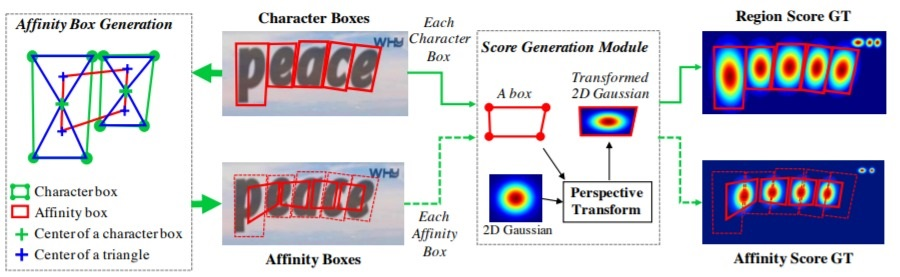
\includegraphics[width=0.9\linewidth]{img/baek}
	\caption{}
	\label{fig:baek}
\end{figure}


Nach dessen Lokalisierung und der daraus gewonnen Koordinaten, werden die gewonnen Informationen in EasyOCR weiterverarbeitet und mittels eines CRNN (Convolutional Recurrent Neural Network) Netzes bestehend aus drei Komponenten ausgelesen. Es handelt sich dabei um eine Feature Extraktion, des Gesuchten Inputs mittels eines ResNets. Eines LSTM (Long-short term memory) Netzes für das sequenzielle Labeling von Charakteren innerhalb eines Wortes. LSTM Netzte eignen sich dabei besonders für die Verarbeitung sequenzieller Daten. Die dritte Komponente besteht aus einem CTC (connection temporal classification) Netz und ist für das Decoding der Outputs innerhalb des LSTM Netzes Zuständig ist \autocite[Vgl.][]{JaidedAI70}. 

Die bei der Praktischen Umsetzung erlangten Resultate sind in dem Folgenden Unterkapitel aufgeführt. Manko bei der jeweiligen Implementierung ist jedoch die Notwendigkeit eines 64Bit Systems für die Implementierung, da die Bibliothek größtenteils auf Pytoch für die Implementierung der Netze zurückgreift. Die Ursprüngliche Hardwarekomponente mittels dessen das Projekt jedoch umgesetzt wird beläuft sich auf ein Rasbery Pi 3. Da für jenen bei der Umsetzung des Projektes (16.12.21-10.02.22) lediglich ein 32Bit Systeme zur Verfügung stand galt es Umsetzung mittels EasyOCR zu verwerfen. Mittlerweile steht jedoch ein 64Bit Systems zur Verfügung, dieses könnten in einer weiterführenden Arbeit die Nutzung des Packages bei Bedürfnis mit der selbigen Hardware erlauben.

Alternativ zu der Erkennung der Schriftzeichen mittels EasyOCR wurde auf die Bibliothek Tesseract 5zurückgegriffen. Diese bedient sich auch eines LSTM Netztes wie die vorherig gesehene Bibliothek, benötigt jedoch keines 64Bit Systems. Tesseract ist dabei ein open source Projekt, dass seit dem Jahr 2005 von Google verwaltet wird und seither immer weiterentwickelt wird. Bei der Umsetzung wird auf $Pytesseract$ und ein vortrainiertes englisches Modell der Texterkennung zurückgegriffen. \autocite[Vgl.][]{Tesserac98}
Bei der Umsetzung wird auch wieder auf ein Preprocessing gesetzt, dass das Bild in Graustufen konvertiert. Des Weiteren wird versucht mittels des Gauß-Verfahrens und gegebenen Filtern, Noise herauszufiltern. Dritter Schritt des Preprocessings ist das hervorhebenden der Kanten mittels der Konvertierung des Bildes in sogenannte $Blobs$, dabei handelt es sich um die Umwandlung eines Graubildes mittels eines festgelegten Schwellenwerts in Binäre Werte. \autocite[Vgl.][]{8974469} 
Das Modell versucht mittels Vektoren Linien auszumachen, auf denen sich die Schriftzüge befinden. Danach geht Tesseract dazu über Zeilenweise Wörter mittels der Bemessung von Abständen auszumachen und Wörter in Bounding-Boxes zu fassen. Die Erkennung der Texte geschieht über das vortrainierte englische LSTM Netzt. Dieses weist bei der Umsetzung jedoch deutlich schlechtere Resultate auf als das zuvor verwendete CRNN (EasyOCR). Die Funktionalität und Genauigkeit beider Modelle wird in einem separaten Kapitel ausgewertet. Da beide Modelle jedoch funktionieren ist es nicht von Nöten das schlechtere zu verwerfen, durch mehrere Versuche das Nummernschild zu lesen gelingt es beiden Modellen das richtige zu lesen. Lediglich die Halbwertszeit ist invers proportional zur Güte der Modelle. Somit ist man auch in der Lage mittels pytesseract die Nummernschild Erkennung durchzuführen und die Resultate mit einer White-list abzugleichen.


\section{Evaluation der Pipelines}

Nach erfolgreichem Proof-of-Concept musste unter den technisch möglichen Varianten der Verarbeitungspipelines die beste ausgewählt werden. Hierzu wurde ein Skript geschrieben, dass die Pipeline in leicht abgewandelter Form für jedes Bild des gesammelten Datensatzes durchführt und das Ergebnis oder eventuelle Fehler in den einzelnen Bearbeitungsschritten festhält. Damit konnten verschiedene OCR-Verfahren untereinander verglichen werden. Ebenso war es möglich die bereits festgestellten Unterschiede in der Bearbeitungsgeschwindigkeit und Qualität von der Berechnung am Laptop gegenüber der Bearbeitung auf dem RasPi zu quantifizieren. Anhand der festgestellten Metriken können schlussendlich auch weiterführende Optimierungen vorgenommen und Fehlerquellen lokalisiert werden.

Die Kennzeichenerkennungspipeline besteht aus folgenden Schritten:

\begin{itemize}
\item Laden der kurz zuvor gespeicherten Datei
\item Preprocessing
\item Umwandlung zu Graustufen
\item Bilateraler Filter
\item Canny-Algorithmus zu Kantenfindung
\item Douglas-Peucker-Algorithmus zur Erkennung von Rechtecken
\item Cropping
\item OCR mit vorgefertigter Lösung
\end{itemize}




Ursprünglich war zu Beginn der Pipeline ein neuronales Netz vorgesehen, mit dem eine erste Eingrenzung des Kennzeichens erfolgen sollte. Dieser Schritt wurde jedoch aufgrund von technischen Problemen entfernt


\subsection{Cropping}
Bei 85 von 118 Bildern wurde eine Region als Kennzeichen identifiziert und freigestellt.
Diese ist nicht immer korrekt, es wurden neben Kennzeichen auch Fenster, Ziegelsteine und Straßenschilder freigestellt.
Das ist ein Problem, das durch die Vorschaltung von yolov3 verhindert werden könnte. 
Eine genauere Evaluation dieses Schrittes ist, ohne die Ergebnisse der nachgeschalteten OCR-Lösung zu berücksichtigen, wenig sinnvoll, weil der Bildausschnitt unvorhersehbare Folgen für das OCR-Ergebnis hat.


\subsection{OCR}
Beide OCR-Lösungen liefern ungenaue Ergebnisse. Die Plaketten zwischen den Blöcken der Kennzeichen werden oft als Zeichen interpretiert. Genauso wird zwischen den Blöcken manchmal ein Leerzeichen erkannt und manchmal nicht.
Bei einem genauen Vergleich dieser Ergebnisse mit einer Liste von erlaubten Kennzeichen würde daher sehr selten ein Treffer auftreten.

Aus diesem Grund wird stattdessen das Python-Paket \lstinline{thefuzz} verwendet, welches sich die Levenshtein-Distanz zu Nutze macht, um die Ähnlichkeit mehrerer Strings zu quantifizieren.
Um die Levenshtein-Distanz zwischen zwei Strings zu bestimmen, wird ein String zum Anderen umgeformt. Erlaubte Operationen sind dabei das Einfügen eines neuen Zeichens und das Entfernen eines bestehenden Zeichens.
Die minimal benötigte Anzahl dieser Operationen ist die Levenshtein-Distanz.

Hieraus wird ein prozentualer Wert abgeleitet, der die Genauigkeit der Erkennung widerspiegelt.
Für die finale Evaluation mit dieser Methode wurde ein Threshold von 45\% gewählt, um das gelesene Kennzeichen als richtig einzuordnen.

Mit easyOCR wurden 28 von 85 Kennzeichen richtig gelesen, mit Tesseract 17.
\begin{figure}[h]
		\centering
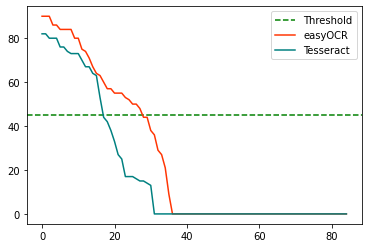
\includegraphics[width=8cm]{./img/evaluation_fuzzy_ratio.png}
\caption{Evaluation mit fuzzy_ratio}
\end{figure}


Neben dem vollständigen Fuzzy Matching können mit der Funktion \lstinline{fuzz.partial_ratio()} auch Substrings berücksichtigt werden.
Das ist sinnvoll, um beispielsweise die Namen von Autohäusern aus den OCR-Ergebnissen herauszufiltern.
Mit dieser Methode (Threshold 45\%) liest easyOCR 31 von 85 Kennzeichen richtig, Tesseract 22. Dies entspricht 26\% bzw. 19\% der Ausgangsmenge von 118 Kennzeichen.
\begin{figure}[h]
		\centering
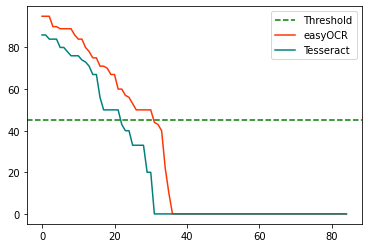
\includegraphics[width=8cm]{./img/evaluation_partial_ratio.png}
\caption{Evaluation mit partial_ratio}
\end{figure}


Abgesehen von den bestehenden Methoden zum Vergleich mehrerer Strings wurde auch ein spezialisierter Ansatz entwickelt. Sowohl easyOCR als auch Tesseract haben die Schwäche, dass sie manchmal die Blöcke der Kennzeichen vertauschen. Um dieses Problem zu umgehen, wurde folgende, auf das vorliegende Problem spezialisierte, Funktion zur Evaluation entwickelt:

% TODO: Formatierung prüfen
\begin{lstlisting} 
	def custom_match(read, label):	
	for x in label:
	if x not in read:
	return 0
	return 100
\end{lstlisting}     
% Bild dazu: eval_custom
Die Werte 0 und 100 dienen der einheitlichen Visualisierung. \lstinline{read} ist der Text, den die OCR-Lösung erkannt hat. \lstinline{label} ist das Label des jeweiligen Bildes in der Form \lstinline{OG AE 1337}. Die leerzeichengetrennten Teile des Labels werden durch Python in jeweils einzelnen Schleifendurchläufen behandelt.
Mit dieser Methode erzielt easyOCR 21 richtige Ergebnisse, Tesseract 5.
\begin{figure}[h]
		\centering
	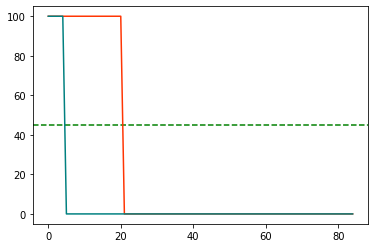
\includegraphics[width=8cm]{./img/evaluation_custom_matcher.png}
	\caption{Evaluation mit eigener Funktion}
\end{figure}


Es ist zu beachten, dass nicht alle im Vorigen Schritt freigestellten Bildsegmente auch wirklich Kennzeichen sind. Ein Mensch könnte an dieser Stelle also auch keine perfekte Leistung erreichen. 

\subsection{Laufzeit}

Für eine praktische Anwendung darf die Laufzeit der gesamten Pipeline nicht zu lang sein.
%Wenn die Laufzeit der Pipeline, also die Verzögerung zwischen der Aufnahme zweier Bilder \delta t ist,
%dann wird das 

Erstens sollte die Zeit zwischen dem Auftauchen des Autos vor der Kamera und dem ersten Scan konsistent sein,
zweitens kann die Pipeline im gleichen Zeitraum mehrmals ausgeführt werden und so trotz ungenauen Modellen gute Ergebnisse erzielen.
Die Laufzeit hängt direkt von der verwendeten Hardware ab.

Zur Evaluation wird die Dauer der einzelnen Schritte (Cropping und OCR) gemessen und zu Durchschnitten aggregiert. 

Auf dem selbst erstellten Datensatz wurde mit einem Lenovo Thinkpad T580 (Intel i7-8850U) für das Cropping durchschnittlich 1,37 Sekunden,
für die Texterkennung mit easyOCR 2,27 Sekunden und für die Bilderkennung mit Tesseract 2,67 Sekunden benötigt.
Das entspricht einer Gesamtlaufzeit von rund 4 Sekunden, also etwa 15 Bildern pro Minute.

Wird jedoch stattdessen ein Raspberry Pi 3 verwendet, steigt die Laufzeit auf durchschnittlich 14,87 Sekunden für das Cropping und 17,62 Sekunden für die Texterkennung mit Tesseract, also insgesamt 32,49 Sekunden.
EasyOCR wurde nicht evaluiert, weil es nicht mit der verwendeten Version von Pi OS kompatibel ist.

Beachtet man, dass das System im schlimmsten Fall kurz vor Ankunft des Fahrzeugs ein Bild aufnahm, so vergehen selbst bei einer direkten Erkennung etwa 60 Sekunden bis zur nächsten Aufnahme und Auswertung. 

\subsection{Zwischenfazit}
Geht man von der besten erreichten Erkennungsrate von 26\% aus, so beträgt der Erwartungswert der benötigten Erkennungsdurchläufe 100/26 = 3,84, welche wiederum 125 Sekunden benötigten. Dazu kommen durchschnittlich 0.5 * 32 Sekunden zur Beendigung der beim Eintreffen ablaufenden Schleife. Die Durchschnittliche Wartedauer beträgt also 141 Sekunden oder 2 Minuten und 21 Sekunden. 
\newline Natürlich ist hier zu beachten, dass beim Warten und der erneuten Bildverarbeitung das Bild ggf. nicht so stark vom vorherigen abweicht wie beim Datensatz und die gleichen Problembereiche hat. Die Erfahrungen im Praxistest auf der Straße lassen aber eher auf eine große Varianz der erkannten Flächen und Texte schließen, weshalb der Wert sich durchaus als Schätzung verwenden lässt.
